\newpage
\subsection{QuizziPedia::Back-End::App}

\label{QuizziPedia::Back-End::App}
\begin{figure}[ht]
	\centering
	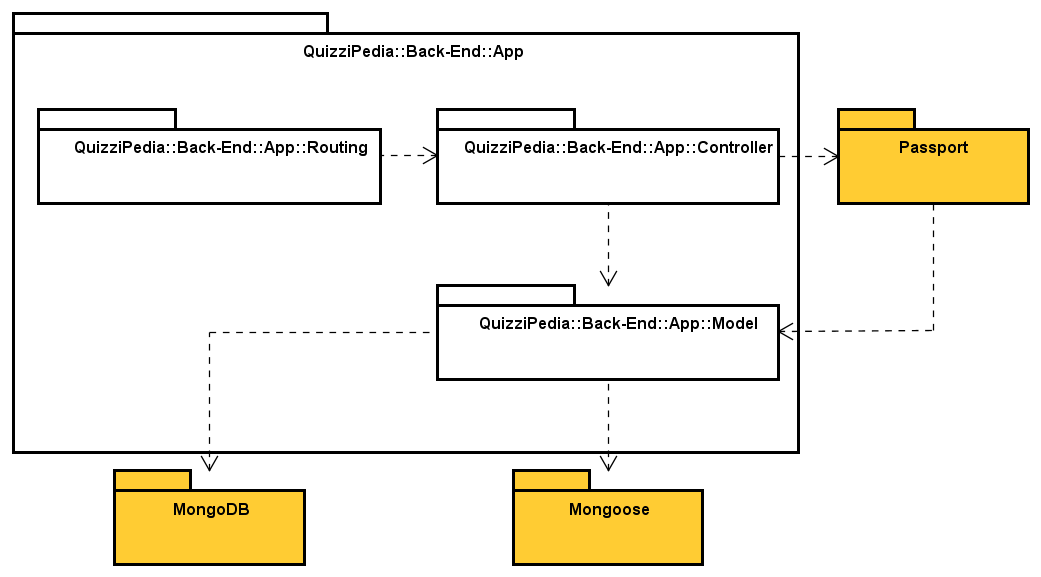
\includegraphics[scale=0.5]{UML/Package/QuizziPedia_Back-End_App.png}
	\caption{QuizziPedia::Back-End::App}
\end{figure}
\FloatBarrier

	\begin{itemize}
		\item \textbf{Descrizione}:
		\textit{package\ped{G}} contenente le componenti del \textit{server\ped{G}} che implementano il \textit{pattern\ped{G} MVC\ped{G}};
		\item \textbf{Padre}: \texttt{Back-End};
		\item \textbf{Interazioni con altri componenti}:
			\begin{itemize}
				\item Config:
				\textit{package\ped{G}} contenente le componenti di configurazione del \textit{server\ped{G}}.
			\end{itemize}
		\item \textbf{Package contenuti}:
			\begin{itemize}
				\item \texttt{Controllers}:
				\textit{package\ped{G}} che contiene i \textit{controllers\ped{G}}  di \textit{Express\ped{G}}, definisce la logica dell'applicazione;
				\item \texttt{Models}:
				\textit{package\ped{G}} che contiene le classi che definiscono il model dell'applicazione. Queste classi cono definite come classi schema di \textit{Mongoose\ped{G}}, il quale permette di utilizzare \textit{MongoDB\ped{G}} tramite degli oggetti;
				\item \texttt{Routers}:
				\textit{package\ped{G}} contenente i \textit{routers} della componente back-end dell'applicazione. Contiene i file di configurazione relativi al routing delle richieste del \textit{client\ped{G}}, ossia i \textit{routers} di \textit{Express\ped{G}}.
			\end{itemize}
	\end{itemize}
	
	\newpage
\subsection{QuizziPedia::Front-End::Controllers}

\begin{figure} [ht]
	\centering
	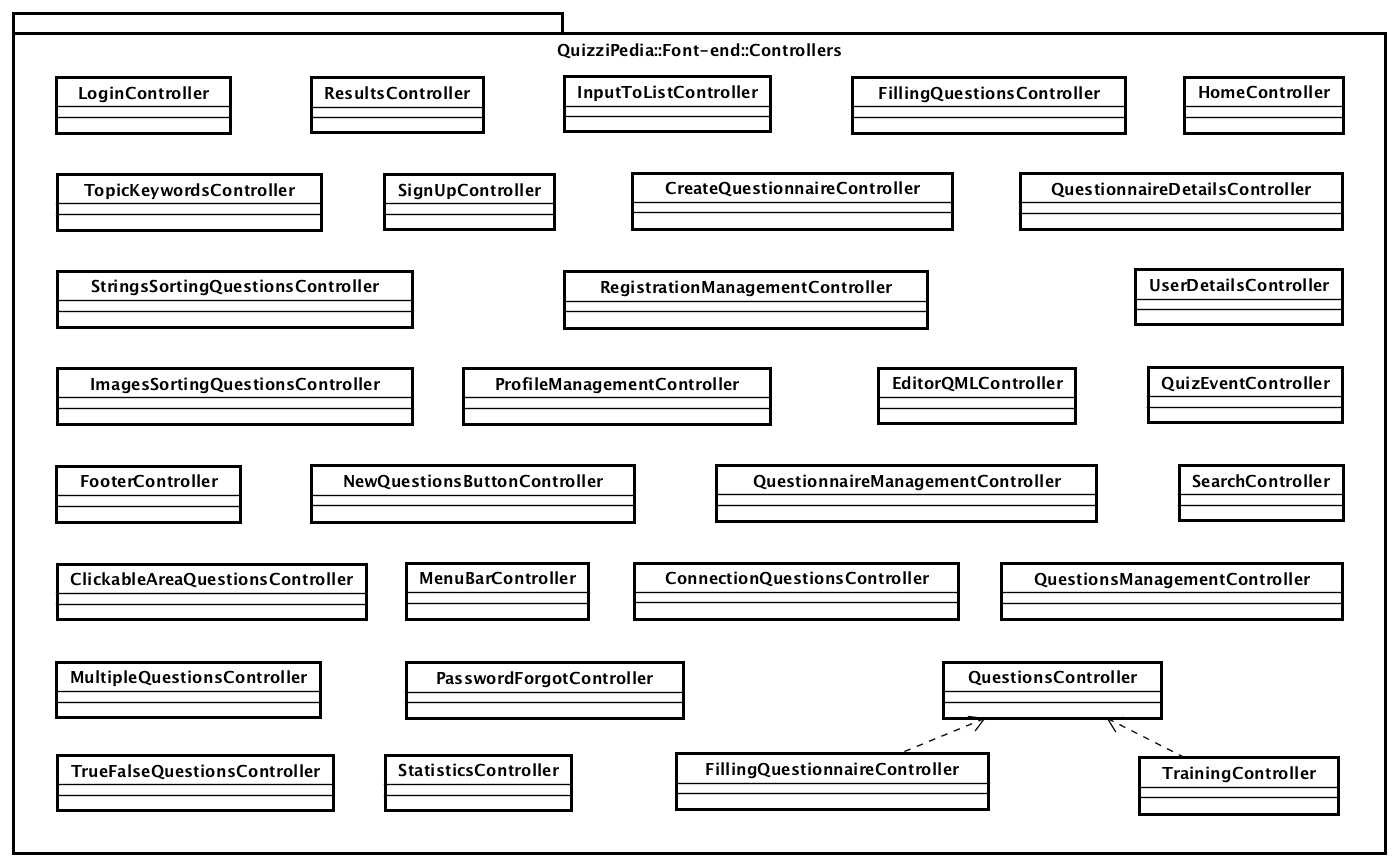
\includegraphics[scale=0.45]{UML/Package/QuizziPedia_Front-End_Controllers.png}
	\caption{QuizziPedia::Front-End::Controllers}
\end{figure} \FloatBarrier

\begin{itemize}
	\item \textbf{Descrizione}: \textit{package\ped{G}} che contiene i controller individuati per la parte front-end dell'applicazione;
	\item \textbf{Padre}: \texttt{Front-End};
	\item \textbf{Interazione con altri componenti}:
	\begin{itemize}
		\item \texttt{Views}: \textit{package\ped{G}} che contiene le \textit{views\ped{G}} dell'applicazione;
		\item \texttt{Models}: \textit{package\ped{G}} che contiene le classi \textit{model\ped{G}} dell'applicazione;
		\item \texttt{Services}: \textit{package\ped{G}} che contiene i \textit{services\ped{G}} dell'applicazione.
	\end{itemize}
	\item \textbf{Classi contenute}:
	\begin{itemize}
		\item \texttt{ClickableAreaQuestionController}: questa classe permette di gestire la creazione e la modifica di una domanda ad area cliccabile;
		\item \texttt{ConnectionQuestionController}: questa classe permette di gestire la creazione e la modifica di una domanda a collegamento;
		\item \texttt{CreateQuesrtionnaireController}: questa classe permette di gestire la creazione di un questionario;
		\item \texttt{EditorQMLController}: questa classe permette di gestire la creazione e la modifica di domande create tramite editor \textit{QML\ped{G}};
		\item \texttt{FillingQuestionnaireController}: questa classe permette di gestire la compilazione del questionario;
		\item \texttt{FillingQuestionsController}: questa classe permette di gestire la creazione e la modifica di una domanda	a riempimento di spazi;
		\item \texttt{HomeController}: questa classe permette di gestire la home page;
		\item \texttt{ImagesSortingQuestionsController}: questa classe permette di gestire la creazione e la modifica di una domanda a ordinamento immagini;
		\item \texttt{InputToListController}: questa classe permette di gestire l'inserimento di una lista di risposte durante la creazione di una domanda;
		\item \texttt{LoginController}: questa classe permette di gestire l'autenticazione dell'utente al sistema;
		\item \texttt{MenuBarController}: questa classe permette di gestire il menù fisso per ogni pagina;
		\item \texttt{MultipleQuestionController}: questa classe permette di gestire la creazione e la modifica di una domanda a risposta multipla;
		\item \texttt{NewQuestionButtonController}: questa classe permette di effettuare il redirect alla pagina di creazione nuova domanda;
		\item \texttt{PasswordForgotController}: questa classe permette di gestire il ripristino della password dimenticata;
		\item \texttt{ProfileManagementController}: questa classe permette di gestire il profilo personale di un utente;
		\item \texttt{QuestionnaireDeatailsController}: questa classe permette di gestire i dettagli di un questionario;
		\item \texttt{QuestionnaireManagementController}: questa classe permette di gestire tutti i questionari creati da un utente;
		\item \texttt{QuestionsController}: questa classe permette di gestire il recupero delle domande per far si che possano essere visualizzate nella modalità allenamento e nella compilazione dei questionari;
		\item \texttt{QuestionsManagementController}: questa classe permette di gestire le domande create dall'utente e di crearne di nuove;
		\item \texttt{QuizEventController}: questa classe permette di reagire ai comandi dell'utente durante la gestione dei suoi questionari;
		\item \texttt{RegistrationManagementController}: questa classe permette di gestire le iscrizione degli utenti ai questionari;
		\item \texttt{ResultQuestionnaireController}: questa classe permette di gestire la visualizzazione dei risultati di un singolo questionario;
		\item \texttt{SearchController}: questa classe permette di gestire la ricerca di questionari e utenti all'interno dell'applicazione;
		\item \texttt{SignUpController}: questa classe permette di gestire la registrazione di un utente al sistema;
		\item \texttt{StatisticsController}: questa classe permette di gestire le statistiche di un utente;
		\item \texttt{StringsSortingQuestionController}: questa classe permette di gestire la creazione e la modifica di una domanda a ordinamento di stringhe;
		\item \texttt{TopicKeywordsController}: questa classe permette di gestire il recupero delle parole chiave di un questionario;
		\item \texttt{TrainingController}: questa classe permette di gestire la modalità allenamento sottoponendo all'utente le giuste domande adatte al suo livello;
		\item \texttt{TrueFalseQuestionController}: questa classe permette di gestire la creazione e la modifica di una domanda	vero/falso;
		\item \texttt{UserDetailsController}: questa classe permette di gestire i dati di un utente da mostrare nella pagina di un profilo.
	\end{itemize} 
\end{itemize}
	\newpage

\subsection{QuizziPedia::Front-End::Models}

	\label{QuizziPedia::Front-End::Models}
	
	\begin{figure}[ht]
		\centering
		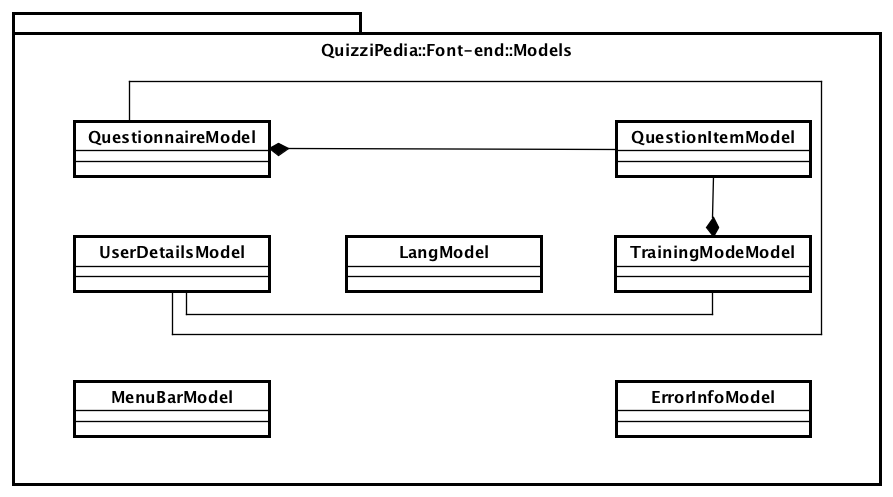
\includegraphics[scale=0.5,keepaspectratio]{UML/Package/QuizziPedia_Front-End_Models.png}
		\caption{QuizziPedia::Front-End::Models}
	\end{figure} \FloatBarrier

		\begin{itemize}
			\item \textbf{Descrizione}: \textit{package\ped{G}} contenente le classi che definiscono la business logic dell'applicazione;
			\item \textbf{Padre}: \texttt{Front-End};
			\item \textbf{Iterazioni con altri componenti}: 
				\begin{itemize}				
					\item \texttt{Controllers}: \textit{package\ped{G}} contenente i controllers front-end dell'applicazione;
					\item \texttt{Directives}: \textit{package\ped{G}} contenente le directives front-end dell'applicazione;
					\item \texttt{Models}: \textit{package\ped{G}} contenente le classi che definiscono la business logic dell'applicazione;
					\item \texttt{Services}: \textit{package\ped{G}} che contiene le classi individuate che permettono la comunicazione del lato front-end con il lato back-end attraverso l'architettura \textit{REST\ped{G}}.
				\end{itemize}
			\item \textbf{Classi contenute}:
			\begin{itemize}
				\item \texttt{UserDetailsModel}: rappresenta un utente. Contiene tutte le informazioni necessarie alla presentazione del contenuto di un utente sia nella visualizzazione che nella gestione di un profilo;
				\item \texttt{TrainingModeModel}: rappresenta un allenamento. Contiene tutte le informazioni necessarie alla presentazione del contenuto di un allenamento;
				\item \texttt{QuestionnaireModel}: rappresenta un questionario. Contiene tutte le informazioni necessarie alla presentazione del contenuto del questionario;
				\item \texttt{QuestionItemModel}: rappresenta una domanda. Contiene tutte le informazioni necessarie alla presentazione del contenuto della domanda;
				\item \texttt{MenuBarModel}: questa classe racchiude i dati necessari per la creazione dinamica della barra menù posizionata in modo fisso su ogni pagina;
				\item \texttt{LangModel}: rappresenta le informazioni per la giusta traduzione dell'applicazione;
				\item \texttt{ErrorInfoModel}: rappresenta le informazioni di un errore che si è verificato eseguendo una determinata operazione;
			\end{itemize}
		\end{itemize}
	\subsubsection{QuizziPedia::Back-End::App::Routers}

\label{QuizziPedia::Back-End::App::Routers}
\begin{figure}[ht]
	\centering
	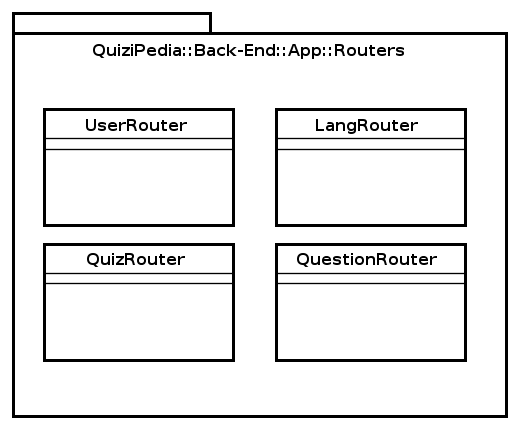
\includegraphics[scale=0.65]{UML/Package/QuizziPedia_Back-End_App_Routers.png}
	\caption{QuizziPedia::Back-End::App::Routers}
\end{figure}
\FloatBarrier
	\begin{itemize}
		\item \textbf{Descrizione}: 
		\textit{package\ped{G}} contenente i router della componente back-end dell'applicazione. Contiene i file di configurazione relativi al routing delle richieste del \textit{client\ped{G}}, ossia i \textit{routers} di \textit{Express\ped{G}};
		\item \textbf{Padre}: \texttt{App};
		\item \textbf{Interazioni con altri componenti}:
			\begin{itemize}
				\item \texttt{Controllers}: \textit{package\ped{G}} che contiene i \textit{Controllers} di \textit{Express\ped{G}}, definisce la logica dell'applicazione.
			\end{itemize}
		\item \textbf{Classi Contenute}:
		\begin{itemize}
			\item \texttt{UserRouter}: classe che gestisce le richieste relative alla registrazione, alla gestione della sessione e alla cronologia dei questionari svolti di un utente. Componente ConcreteHandler del design pattern \textit{Chain of responsibility\ped{G}}. Utilizza il modulo \textit{Passport\ped{G}};
			\item \texttt{QuestionRouter}: classe che gestisce le richieste relative alle operazioni riguardanti le domande. Componente ConcreteHandler del design pattern \textit{Chain of responsibility\ped{G}}. Utilizza il modulo \textit{Passport\ped{G}};
			\item \texttt{QuizRouter}: classe che gestisce le richieste relative alle operazioni riguardanti un questionario;
			\item \texttt{LangRouter}: classe che gestisce le richieste relative alla lingua;
		\end{itemize}
	\end{itemize}
